%*******************************************************************************
%*********************************** Third Chapter *****************************
%*******************************************************************************

\chapter{Fine-grained Recognition}
\label{chap:finegrained_classification}

%% Write about Paper A and B in a coherent way

This chapter presents an approach for enhancing fine-grained classification performance of grocery items by using web-scraped information. We focus on classification of grocery items due to applicability in assistive vision and its potential to enhance the independence of visually impaired (VI) people [ADD groceries/shopping/object recognition for VI REFs]. Initially, we were interested in learning classifiers with natural images taken in the grocery stores combined with web-scraped information about the grocery items, such as iconic images and text descriptions from supermarket websites. Using iconic images have been used in grocery image classification earlier [ADD grocery paper REFs], however, utilizing text descriptions was as far we know absent for this application even if it has been successfully applied in other image classification problems~\cite{wah2011cub, nilsback2008automated, bujwid2021large}. Thus, we collected our own dataset of grocery items images using a mobile phone camera as well as web-scraped images and text descriptions to study whether this multi-view approaches would benefit training the classifiers (Section 2). We then select a multi-view learning framework based on the Variational Autoencoder (VAE) for investigating how the different data views affect the fine-grained classification performance (Section 3). 

%\section{Introduction}
\section{Related Work}

In this section, we will briefly discuss the related work on fine-grained image recognition~\cite{wei2021fine}, particularly when learning from external information, and multi-view learning. 

\subsection{Fine-grained Image Recognition}
%\paragraph{Fine-grained Image Recognition.} 
The goal with fine-grained image recognition (FGIR) is to distinguish between images with multiple visually similar sub-categories that belong to a super-category. For example, various attempts have been made to discriminate between sub-categories of different animals~\cite{van2018inaturalist}, cars~\cite{krause2013stanford_cars}, fruits~\cite{hou2017vegfru}, retail products~\cite{wei2019rpc}, etc. The challenge is to recognize differences that are sufficient for discriminating between objects that are generally similar but differ in fine-grained visual details. In recent years, the successes with deep learning in computer vision have encouraged researchers to explore various approaches for FGIR that can broadly be divided into three directions for recognition by utilizing (i) localization-classification subnetworks, (ii) end-to-end feature encoding, and (iii) external information. In (i), the goal is to find object parts that are shared across the sub-categories for discovering details that make the part representations different. This can be achieved by utilizing feature maps from the activations of convolutional layers as local descriptors~\cite{zhang2016picking, wang2018learning, ding2019selective}, employing detection and segmentation techniques for localizing object parts[REFs], or leveraging attention mechanisms when common object parts are difficult to represent or even define [REFs]. With (ii), the goal has been to learn features that are better at capturing subtle and local differences by, for instance, performing high-order features interactions~\cite{lin2015bilinear} as well as designing novel loss functions [Add REFs]. In the third approach (iii), the goal is to leverage external information, for example, web data and multimodal data, in FGIR as additional supervision to the images. We will put more focus on the approach on FGIR with external information next, as we use this approach in Paper A and B. 

\subsection{Recognition with External Information}
%\paragraph{Recognition with External Information.} 
Learning fine-grained details about objects often requires large amounts of labeled data. To ease the need for large amounts of accurately labeled images, there have been several attempts to let either web-scraped or multimodal data influence learning the fine-grained features of the sub-categories to boost the FGIR performance. Web-scraped images may be noisy in the sense that retrieved images may have high-variations of the objects. For example, the objects of interest can look different in appearance, and there could also be other irrelevant objects in the images that potentially occlude the category to recognize. Hence, incorporating web-scraped data into the training set may establish a domain gap between the easily acquired web data and the original training set which we need to overcome by reducing the domain gap or reducing the negative effects of the noisy web data that can disturb the learning. Another direction than using web-scraped data is to utilize multimodal data, for example, images, text and knowledge bases, for boosting the classification performance. In FGIR, the goal is to establish a joint representation between the images and additional data sources, where the additional data should act like extra guidance for learning useful representations that capture the fine-grained details of objects. Text descriptions have been a popular data type to combine with images, which can be both easy and cheap to collect as they can be accurately generated by non-experts. High-level knowledge graphs of objects have also been used and can contain rich knowledge useful for fine-grained recognition. In addition to FGIR, both web-scraped and multimodal external information has been used for zero-shot learning to transfer knowledge from annotated categories to new fine-grained categories. In Paper A, we collect web-scraped images and text descriptions of grocery items to accompany real-world images of groceries for FGIR. Then, in Paper B, we perform a study using multi-view learning to investigate how the external information can enhance the classification performance. Next, we will cover the related work for the multi-view learning approach that we used. 


\subsection{Multi-view Learning}
%\paragraph{Multi-view Learning.} 
\MK{TO-DO: Learning from several data sources and modalities. Briefly on multi-view learning approchaes and VCCA.} % CCA, Autoencoders, VCCA, multimodal VAEs



%There exist lots of multi-view learning approaches for data fusion of multiple features~\cite{baltruvsaitis2018multimodal, cremer2018importance, frome2013DeVISE, fu2016semi, karpathy2015deep, ngiam2011multimodal, pieropan2014audio,  salzmann2010factorized, shi2019variational, suzuki2016joint, tsai2018learning, vedantam2017generative, wang2016deep, wu2018multimodal, xian2018zero, xu2013survey, zhang2016inter, zhao2017multi}. A common approach is to obtain a shared latent space for all views with the assumption that each view has been generated from this shared space~\cite{xu2013survey}. A popular example of this is approach is Canonical Correlation Analysis (CCA)~\cite{hotelling1936relations}, which aims to project two sets of variables (views) into a lower-dimensional space so that the correlation between the projections is maximized. Similar methods propose maximizing other alignment objectives for embedding the views, such as ranking losses~\cite{frome2013DeVISE, fu2016semi, karpathy2015deep, xian2018zero}. 
%There exist nonlinear extensions of CCA, e.g., Kernel CCA~\cite{akaho2006kernel} and Deep CCA~\cite{andrew2013deep}, that optimize their nonlinear feature mappings based on the CCA objective. 
%Deep Canonically Correlated Autoencoders (DCCAE)~\cite{wang2015deep} is a Deep CCA model with an autoencoding part, which aims to maximize the canonical correlation between the extracted features as well as reconstructing the input data. 
%Removing the CCA objective reduces DCCAE to a standard multi-view autoencoder, e.g., Bimodal Autoencoders and Split Autoencoders (SplitAEs)~\cite{ngiam2011multimodal, wang2015deep}, that only aim to learn a representation that best reconstructs the input data. SplitAEs aim to reconstruct two views from a representation encoded from one of the views. This approach was empirically shown to work better than Bimodal Autoencoders in \cite{ngiam2011multimodal} in situations where only a single view is present at both training and test time.

%Variational CCA (VCCA)~\cite{wang2016deep} can be seen as an extension of CCA to deep generative models, but can also be described as a probabilistic version of SplitAEs.
%VCCA uses the amortized inference procedure from Variational Autoencoders (VAEs)~\cite{kingma2013auto, zhang2018advances} to learn the shared latent space by maximizing a lower bound on the data log-likelihood of the views. Succeeding works have proposed new learning objectives and inference methods for enabling conditional generation of views, e.g., generating an image conditioned on some text and vice versa~\cite{cremer2018importance, shi2019variational, suzuki2016joint, vedantam2017generative, wu2018multimodal}. These approaches rely on fusing the views into the shared latent space as the inference procedure, which often requires tailored training and testing paradigms when views are missing. However, adding information from multiple views may not lead to improved results and can even make the model perform worse on the targeted task~\cite{guler2014whats, ngiam2011multimodal}. This is especially the case when views have noisy observations, which complicates learning a shared latent space that combines the commonalities between the views. To avoid disturbing the shared latent space with noise from single views, some works design models which extend the shared latent space with private latent spaces for each view that should contain the view-specific variations to make learning the shared variations easier~\cite{hyvarinen2000independent, salzmann2010factorized, tsai2018learning, wang2016deep, zhang2016inter}. VCCA can be extended to extract shared and private information between different views through factorization of the latent space into shared and private parts. In this paper, we investigate if the classification performance of grocery items in natural images can be improved by extracting the view-specific variations in the additional views (iconic images and product descriptions) from the shared latent space with this variant of VCCA called VCCA-private. We will experiment with treating each data point as pairs of natural images and either iconic images or text descriptions as well as triplets of natural images, iconic images, and text descriptions.
%A difference between how we apply VCCA to our dataset compared to the works above is that the iconic image and text description are the same for every natural image of a specific class.  



%Adding web-scraped data of the categories of interest to the training data is referred to as \textit{webly supervised learning}  

%There have been several attempts to utilize external information, for example, web images, to enhance the performance of FGIR. % How are we different from other works that used web information for recogntion? This can be on dataset level. But also describe some approaches and then that we use multi-view learning. 


\section{Dataset Collection}
In this section, we describe our procedure for collecting the image dataset of grocery items. As the target use case is grocery shopping with an assistive vision device, we visited several supermarkets and collected natural images of the groceries with a mobile phone camera to imitate such scenarios. Hence, the collected images will capture situations that can be challenging for the assistive device, such as, various lighting conditions, multiple instances and classes present, hand occlusions, and misplaced items. All images were taken with a single targeted item in mind, such that each image is paired with a single label. For items which belong to a clear super-class, for example, various kinds of apples and milk packages, we also provided the general class of the items to establish a hierarchical labeling structure of the data. Collecting natural images of the grocery items is unfortunately a time-consuming process. Furthermore, as the surroundings in every grocery store varies, it may be difficult to build accurate classifiers that can recognize fine-grained details solely from natural images. Hence, we need some cheaper procedure that can complement the collection of real-world images for boosting the classification performance of the groceries. 

We have complemented the image dataset with external information from the web of each grocery item that can be used for training classifiers. In the past years, most supermarket chains have the option for consumers to purchase groceries online from their websites. The website usually provides each grocery item with an iconic image of the item on a white background, a text description that describes the flavor and ingredients of the item, as well as nutrition values if applicable. We downloaded these information types of all grocery item classes by web-scraping the online shopping website of a supermarket chain. We show four examples of grocery items and their web-scraped information in Table \ref{tab:grocery_store_dataset}. Since these data types are on a class-based level, we can use the web-scraped information as weak supervision to guide the classifier to learn fine-grained details that helps discriminating between visually similar items.   

\begin{table}[t]
	\centering
	\caption{\small{ Examples of grocery item classes in the Grocery Store dataset. We display four different items (coarse-grained class in parenthesis), followed by two natural images taken with a mobile phone inside grocery stores. Next comes the web-scraped information of the items consisting of an iconic image and a text description. We have highlighted ingredients and flavors in the text description that are characteristic for the specific item. }}
	\vspace{-10pt}
	\setlength{\fboxsep}{0pt} 
	\setlength{\fboxrule}{0.33pt}
	

	%\resizebox{0.98\textwidth}{!}{
	\begin{tabular}{c | c | c | c}
	\hline
	\thead{\footnotesize Class \\ \footnotesize Labels} & \thead{\footnotesize Natural \\ \footnotesize Images} & \thead{\footnotesize Iconic \\ \footnotesize Images} & \thead{\footnotesize Text \\ \footnotesize Descriptions} \\
	\hline 
	\makecell{ \scriptsize Granny Smith \\[-1pt] \scriptsize (Apple)}
	&  \makecell{ \begin{tikzpicture}
			\begin{scope}
				\node {\fbox{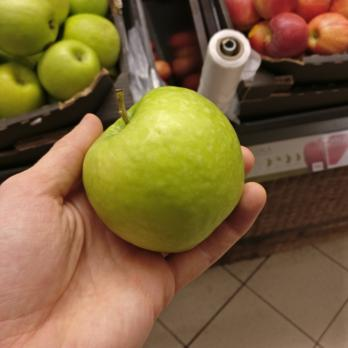
\includegraphics[width=30pt]{Chapter1/pics/Granny-Smith_021.jpg}}};
			\end{scope}
			\begin{scope}[xshift=34pt]
				\node {\fbox{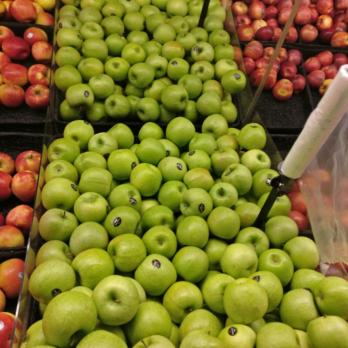
\includegraphics[width=30pt]{Chapter1/pics/Granny-Smith_012.jpg}}};
			\end{scope}
	\end{tikzpicture} }& 
	\makecell{\begin{tikzpicture}
			\begin{scope}
				\node {\fbox{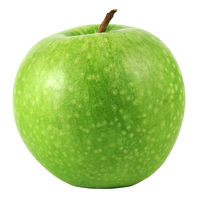
\includegraphics[width=30pt]{Chapter1/pics/Granny-Smith_Iconic.jpg}}};
			\end{scope}
	\end{tikzpicture} } & 
	\begin{scriptsize}
		\makecell{ \textit{“…green apple with white, firm pulp } \\[-1pt]  \textit{and a clear acidity in the flavor.”} } 
	\end{scriptsize}
	\\
	\hline 
	\makecell{ \scriptsize Royal Gala \\[-1pt] \scriptsize (Apple)}
	&  \makecell{ \begin{tikzpicture}
			\begin{scope}
				\node {\fbox{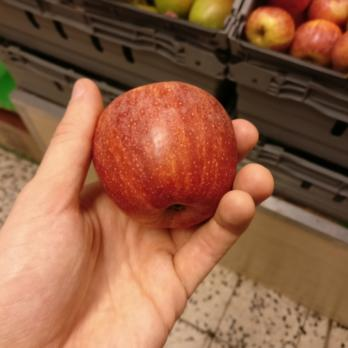
\includegraphics[width=30pt]{Chapter1/pics/Royal-Gala_005.jpg}}};
			\end{scope}
			\begin{scope}[xshift=34pt]
				\node {\fbox{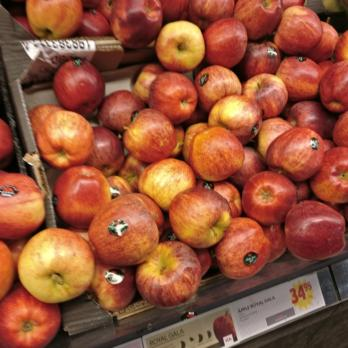
\includegraphics[width=30pt]{Chapter1/pics/Royal-Gala_002.jpg}}};
			\end{scope}
	\end{tikzpicture} }& 
	\makecell{\begin{tikzpicture}
			\begin{scope}
				\node {\fbox{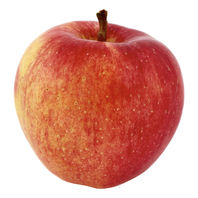
\includegraphics[width=30pt]{Chapter1/pics/Royal-Gala_Iconic.jpg}}};
			\end{scope}
	\end{tikzpicture} } & 
	\begin{scriptsize}
		\makecell{ \textit{“…crispy and very juicy apple,} \\[-1pt] \textit{with yellow-white pulp. The peel} \\[-1pt] \textit{is thin with a red yellow speckled color.”} } 
	\end{scriptsize}
	\\
	\hline
	\makecell{ \scriptsize Tropicana \\[-1pt] \scriptsize Mandarin \\[-1pt] \scriptsize (Juice)}
	&  \makecell{ \begin{tikzpicture}
			\begin{scope}
				\node {\fbox{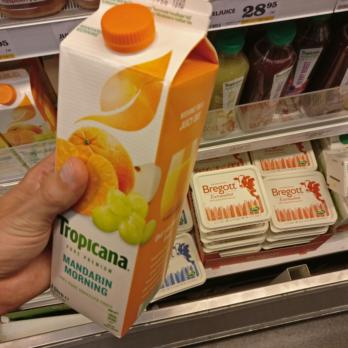
\includegraphics[width=30pt]{Chapter1/pics/Tropicana-Mandarin-Morning_003.jpg}}};
			\end{scope}
			\begin{scope}[xshift=34pt]
				\node {\fbox{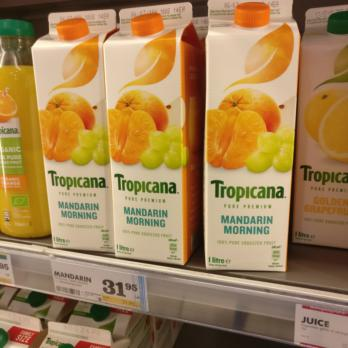
\includegraphics[width=30pt]{Chapter1/pics/Tropicana-Mandarin-Morning_016.jpg}}};
			\end{scope}
	\end{tikzpicture} }& 
	\makecell{\begin{tikzpicture}
			\begin{scope}
				\node {\fbox{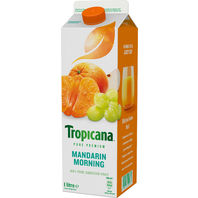
\includegraphics[width=30pt]{Chapter1/pics/Tropicana-Mandarin-Morning_Iconic.jpg}}};
			\end{scope}
	\end{tikzpicture} } & 
	\begin{scriptsize}
		\makecell{ \textit{“…is a ready to drink juice} \\[-1pt]
			\textit{without pulp pressed on orange,} \\[-1pt]
			\textit{ mandarin and grapes. Not from} \\[-1pt]
			\textit{concentrate. Mildly pasteurized.” } }
	\end{scriptsize}
	\\
	\hline
	\makecell{ \scriptsize Yoggi Vanilla \\[-1pt] \scriptsize (Yoghurt)}
	&  \makecell{ \begin{tikzpicture}
			\begin{scope}
				\node {\fbox{
\includegraphics[width=30pt]{Chapter1/pics/Yoggi-Vanilla-Yoghurt_001.jpg}}};
			\end{scope}
			\begin{scope}[xshift=34pt]
				\node {\fbox{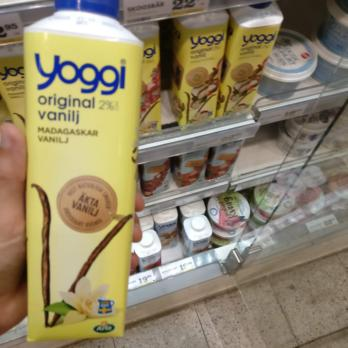
\includegraphics[width=30pt]{Chapter1/pics/Yoggi-Vanilla-Yoghurt_010.jpg}}};
			\end{scope}
	\end{tikzpicture} }& 
	\makecell{\begin{tikzpicture}
			\begin{scope}
				\node {\fbox{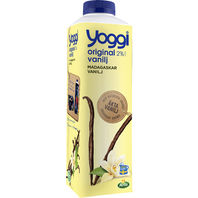
\includegraphics[width=30pt]{Chapter1/pics/Yoggi-Vanilla-Yoghurt_Iconic.jpg}}};
			\end{scope}
	\end{tikzpicture} } & 
	\begin{scriptsize}
		\makecell{ \textit{“...creamy vanilla yoghurt} \\[-1pt]
			\textit{original... added sugar than  } \\[-1pt]
			\textit{regular flavored yoghurt. Great for } \\[-1pt]
			\textit{both breakfast and snacks.”}}
	\end{scriptsize}
	\\
	\hline
\end{tabular}
%}
	\label{tab:grocery_store_dataset}
	%\vspace{-7mm}
\end{table}

\section{Fine-grained Classification of Grocery Items}

This section describes the approaches we used for classification of grocery items from the available data types in the collected dataset. We begin by introducing the problem setting, followed by describing the methods for learning representations from the available data views. 

\subsection{Problem Setting}

The application we are focusing on is grocery shopping with an assistive vision device. The device could for instance be a mobile phone app where the groceries are recognized by an in-built image classifier from natural images taken with the camera. Training such image classifier to be robust in grocery store environments would typically require an immense amount of labeled training examples of all available groceries. To reduce the need for labeled training data, we aim to combine the collected natural images with web-scraped information about the groceries when training the classifier. The goal is that incorporating the web-scraped information should help the classifier to learn fine-grained details about the items to enhance the classification performance and robustness. 

The available data views that are available for training image classifiers is denoted as follows:
\begin{itemize}[itemsep=0em,topsep=1pt]
	\item $\vx$: Natural images of the grocery items in the grocery stores.
	\item $\vy$: Class labels of grocery items from corresponding natural images.
	\item $\vi$: Iconic images of the grocery items scraped from a supermarket website.
	\item $\vw$: Text description of the grocery items scraped from the same supermarket website as $\vi$.
\end{itemize}
The simplest approach is to take a standard supervised approach and train a CNN from the natural image and class label pairs. An alternative is leverage from CNNs pre-trained on a large dataset, such as Imagenet~\cite{deng2009imagenet}, and fine-tune the final classification layer to the grocery item recognition task~\cite{sharif2014cnn}. We use ideas from multi-view learning~\cite{xu2013survey} and VAEs~\cite{kingma2013auto} for learning joint representations from the available data views that can be used for training the image classifiers, which we present in the next section.  


\subsection{Multi-view Representation Learning of Grocery Items}

This section describes the approach we took for learning representations of grocery items that are shared across the available data types. We employ a deep latent variable model called Variational Canonical Correlation Analysis~\cite{wang2016deep} (VCCA) for learning the shared representation. The main assumption in VCCA is that each data view have been generated from the same latent space. The goal then is to learn this latent space that captures the correspondences between all views into representations shared across the views for the grocery items. This representation can then be utilized for enhance the learning more accurate classifiers as well as for performing tasks such as synthesis and prediction of novel images. Next, we describe how to enable learning the shared latent space. 

Capturing variations from each view in the learned representation is performed by predicting the original views from the latent space. To obtain the latent representation, we extract the representation by encoding the natural images with neural network. The extracted representation is then used for predicting each view individually by inputting the representation through separate neural networks. Note that we only use the natural images for extracting the latent representation here since it is the only view that is available at test time when we want to use the learned classifier in the grocery store. We have two options for exploiting the new representation to train classifiers. The first option is to train the classifier with the latent representations after we have learned the latent space as described above. The second option is to train the classifier and learning the latent space simultaneously by adding an additional classifier network predicting the class label with the latent representation as input. 

\MK{TO-DO: I should add a figure of the architecture for extra clarity on the method. }
%The architecture that we used is shown in Figure X. 



%we take an encoder-decoder approach as these have been successful in applications with data with images and class-specific additional data types. this is in contrast to webly supervised methods where the web data usually has many instances per class. 

%we use shared subspace learning approach from multi-view learning because it is a simple approach that gives us a joint representation across the views that we can use for training classifiers. This also opens up for using generative modeling approaches 


\section{Experiments}

In this section, we summarize the main results from the experimental study in Paper B. We performed an ablation study with VCCA over the combinations of available data views to investigate how each data view contributes to the classification performance. First, we present results on fine-grained classification performance between the compared methods. Then, we provide insights in how the web-scraped icnoc images and text descriptions contribute to the boosting the classification performance by visualizing their the joint latent spaces. Finally, we demonstrate how the iconic image decoder in VCCA can be used for explaining the misclassifications by generating iconic images from natural images at test time. 

We compare the VCCA models against two CNN baselines that uses the DenseNet~\cite{huang2017densely} architecture. The first baseline is a DenseNet trained from scratch on the dataset, and the second baseline is a Softmax classifier trained from image features extracted from a DenseNet pre-trained on ImageNet. We denote which data views that are used by VCCA using subscripts. For instance, VCCA$_{\vx \vi \vw}$ means that the natural images $\vx$, iconic images $\vi$, and text descriptions $\vw$ are utilized for learning the joint latent representation. These VCCA models uses the two-stage classifier setup with steps 1) train VCCA on the data views, and 2) train 1-layer MLP classifier using the extracted latent representations from VCCA and the corresponding class labels. We also compare against VAE$_{\vx}$ only using the natural images $\vx$ trained in this setting. The VCCA models with class label decoders are denoted by using $\vy$ in the subscript, such as VCCA$_{\vx \vi \vw \vy}$. 

\begin{figure}[t]
	\centering
	\setlength{\figwidth}{0.62\textwidth}
	\setlength{\figheight}{.22\textheight}
	% This file was created with tikzplotlib v0.10.1.

\pgfplotsset{compat=1.11,
	/pgfplots/ybar legend/.style={
		/pgfplots/legend image code/.code={%
			\draw[##1,/tikz/.cd,yshift=-0.25em]
			(0cm,0cm) rectangle (3pt,0.8em);},
	},
}

\begin{tikzpicture}
	
\tikzstyle{every node}=[font=\footnotesize]

\definecolor{crimson2143940}{RGB}{214,39,40}
\definecolor{darkgray176}{RGB}{176,176,176}
\definecolor{darkorange25512714}{RGB}{255,127,14}
\definecolor{forestgreen4416044}{RGB}{44,160,44}
\definecolor{lightgray204}{RGB}{204,204,204}
\definecolor{mediumpurple148103189}{RGB}{148,103,189}
\definecolor{orchid227119194}{RGB}{227,119,194}
\definecolor{steelblue31119180}{RGB}{31,119,180}

\begin{axis}[
height=\figheight,
legend cell align={left},
legend columns=2,
legend style={
  fill opacity=0.8,
  draw opacity=1,
  text opacity=1,
  at={(1.02,0.97)},
  anchor=north west,
  draw=lightgray204,
  font=\scriptsize
},
minor xtick={},
minor ytick={62.5,67.5,72.5,77.5},
tick align=outside,
width=\figwidth,
x grid style={darkgray176},
xlabel={},
xmajorticks=false,
xmin=-0.725, xmax=9.725,
xtick style={color=black},
xtick={-2,0,2,4,6,8,10},
y grid style={darkgray176},
ylabel={Accuracy (\%)},
yminorgrids,
ymajorgrids,
ymin=59, ymax=81,
ytick pos=left,
ytick style={color=black},
ytick={60,65,70,75,80},
yticklabels={60,65,70,75,80}
]
\draw[draw=black,fill=steelblue31119180,opacity=0.85] (axis cs:-0.25,0) rectangle (axis cs:0.25,67.33);
\addlegendimage{ybar,ybar legend,draw=black,fill=steelblue31119180,opacity=0.85}
\addlegendentry{DenseNet}

\draw[draw=black,fill=darkorange25512714,opacity=0.85] (axis cs:0.75,0) rectangle (axis cs:1.25,71.67);
\addlegendimage{ybar,ybar legend,draw=black,fill=darkorange25512714,opacity=0.85}
\addlegendentry{Softmax}

\draw[draw=black,fill=forestgreen4416044,opacity=0.85] (axis cs:1.75,0) rectangle (axis cs:2.25,69.2);
\addlegendimage{ybar,ybar legend,draw=black,fill=forestgreen4416044,opacity=0.85}
\addlegendentry{VAE$_{\vx}$}

\draw[draw=black,fill=forestgreen4416044,opacity=0.85,postaction={pattern=north east lines, fill opacity=0.85}] (axis cs:2.75,0) rectangle (axis cs:3.25,70.72);
\addlegendimage{ybar,ybar legend,draw=black,fill=forestgreen4416044,opacity=0.85,postaction={pattern=north east lines, fill opacity=0.85}}
\addlegendentry{VCCA$_{\vx \vy}$}

\draw[draw=black,fill=crimson2143940,opacity=0.85] (axis cs:3.75,0) rectangle (axis cs:4.25,77.02);
\addlegendimage{ybar,ybar legend,draw=black,fill=crimson2143940,opacity=0.85}
\addlegendentry{VCCA$_{\vx \vi}$}

\draw[draw=black,fill=crimson2143940,opacity=0.85,postaction={pattern=north east lines, fill opacity=0.85}] (axis cs:4.75,0) rectangle (axis cs:5.25,77.22);
\addlegendimage{ybar,ybar legend,draw=black,fill=crimson2143940,opacity=0.85,postaction={pattern=north east lines, fill opacity=0.85}}
\addlegendentry{VCCA$_{\vx \vi \vy}$}

\draw[draw=black,fill=mediumpurple148103189,opacity=0.85] (axis cs:5.75,0) rectangle (axis cs:6.25,75.37);
\addlegendimage{ybar,ybar legend,draw=black,fill=mediumpurple148103189,opacity=0.85}
\addlegendentry{VCCA$_{\vx \vw}$}

\draw[draw=black,fill=mediumpurple148103189,opacity=0.85,postaction={pattern=north east lines, fill opacity=0.85}] (axis cs:6.75,0) rectangle (axis cs:7.25,74.72);
\addlegendimage{ybar,ybar legend,draw=black,fill=mediumpurple148103189,opacity=0.85,postaction={pattern=north east lines, fill opacity=0.85}}
\addlegendentry{VCCA$_{\vx \vw \vy}$}

\draw[draw=black,fill=orchid227119194,opacity=0.85] (axis cs:7.75,0) rectangle (axis cs:8.25,77.51);
\addlegendimage{ybar,ybar legend,draw=black,fill=orchid227119194,opacity=0.85}
\addlegendentry{VCCA$_{\vx \vi \vw}$}


\draw[draw=black,fill=orchid227119194,opacity=0.85,postaction={pattern=north east lines, fill opacity=0.85}] (axis cs:8.75,0) rectangle (axis cs:9.25,77.78);
\addlegendimage{ybar,ybar legend,draw=black,fill=orchid227119194,opacity=0.85,postaction={pattern=north east lines, fill opacity=0.85}}
\addlegendentry{VCCA$_{\vx \vi \vw \vy}$}

\path [draw=black, semithick]
(axis cs:0,65.98)
--(axis cs:0,68.68);

\path [draw=black, semithick]
(axis cs:1,71.39)
--(axis cs:1,71.95);

\path [draw=black, semithick]
(axis cs:2,68.74)
--(axis cs:2,69.66);

\path [draw=black, semithick]
(axis cs:3,70.16)
--(axis cs:3,71.28);

\path [draw=black, semithick]
(axis cs:4,76.51)
--(axis cs:4,77.53);

\path [draw=black, semithick]
(axis cs:5,76.67)
--(axis cs:5,77.77);

\path [draw=black, semithick]
(axis cs:6,74.91)
--(axis cs:6,75.83);

\path [draw=black, semithick]
(axis cs:7,73.87)
--(axis cs:7,75.57);

\path [draw=black, semithick]
(axis cs:8,77)
--(axis cs:8,78.02);

\path [draw=black, semithick]
(axis cs:9,77.33)
--(axis cs:9,78.23);

\end{axis}

\end{tikzpicture}

	\vspace{-2mm}
	\caption{Fine-grained accuracies on the Grocery Store dataset for all classification methods. We show the means and standard deviations averaged over 5 seeds. Adding the iconic image $\vi$ and text description $\vw$ for learning joint representations with VCCA improves the classification performance over approaches that only utilize the natural images and class labels.}
	\label{fig:fine_grained_classification_results}
	\vspace{-4mm}
\end{figure}

\paragraph{Fine-grained Classification Results.} Adding the web-scraped views in VCCA improves the classification performance over approaches that only utilize the natural images and class labels. Figure \ref{fig:fine_grained_classification_results} shows a bar plot over the fine-grained accuracies achieved by all classification methods. Among the methods only using natural images and class labels, we see that the Softmax baseline performs best, which could be due to some information loss when compressing the images into as low-dimensional latent representations with VAE$_{\vx}$ and VCCA$_{\vx \vy}$. The performance of VCCA significantly improves over Softmax when the iconic image $\vi$ and text description $\vw$ are used, which shows that both data views are useful for enhancing the fine-grained classification performance. Comparing VCCA$_{\vx \vi}$ and VCCA$_{\vx \vw}$, we see that utilizing the iconic image has an advantage over using the text description for improving the performance. This could be due to the fact that the text descriptions are providing information on ingredients and flavors rather than visual appearance. Combining both $\vi$ and $\vw$ achieves on par performance as only utilizing the iconic image, which could potentially be improved by filtering the text descriptions for obtaining words relevant for describing the fine-grained details of the items. Finally, we observe that both classification options for VCCA performs similar, which could potentially be since $\vi$ and $\vw$ acts as labels since there is only a single instance of these views for all classes.  



\paragraph{Visualization of Latent Space.} The web-scraped iconic images and text descriptions structures the grocery items based on view-specific similarities in the latent space that are beneficial for fine-grained classification. In Figure \ref{fig:latent_space_visualizations}, we illustrate how adding either the iconic image $\vi$ or the text description $\vw$ changes the structure of the latent space, where we have used PCA to project the latent representations into a 2-dimensional space. In Figure \ref{fig:latent_space_visualizations}(a-c), we have plotted the corresponding iconic image for all latent representations of models VAE$_{\vx}$, VCCA$_{\vx \vi}$, VCCA$_{\vx \vw}$ for visualization purposes. The latent space for VAE$_{\vx}$ separates raw and packaged grocery items into two separate clusters. When adding the iconic image in VCCA$_{\vx \vi}$, we observe that the latent space becomes structured according to the color of the items. For VCCA$_{\vx \vw}$, the latent space becomes structured according to the ingredients of the items, where we see in the raw food cluster that bell peppers are placed in the upper region while apples are in the lower region. 

Next, we focus on a certain set of classes to inspect to gain more insights in how the additional data views affect the latent space. First, we focus on the green and red apples classes to inspect how the views handle visually different items in color. In Figure \ref{fig:latent_space_visualizations}(d-f), we plot the latent representations for the three models but highlight the green and red apple classes by plotting them as green and red dots respectively. All other classes are plotted as smaller blue dots. We see that both VCCA$_{\vx \vi}$ and VCCA$_{\vx \vw}$ manages to separate the apple classes better than VAE$_{\vx}$, where adding the iconic images yields the most clear separation. Next, we want to study the benefits of the text descriptions. We focus on some yoghurt and juice package classes that are visually similar but have very different ingredients and flavors. In Figure \ref{fig:latent_space_visualizations}(g-i), we plot the latent representations for the three models again where the yoghurt and juice classes are plotted in green and yellow colored dots respectively. Here, we see that VCCA$_{\vx \vw}$ manages to separate these items better than VCCA$_{\vx \vw}$ due to the differences in the text descriptions between the selected package classes. 

\begin{figure}[t]
	\centering
	
\begin{subfigure}[b]{0.3\textwidth}
	\centering
	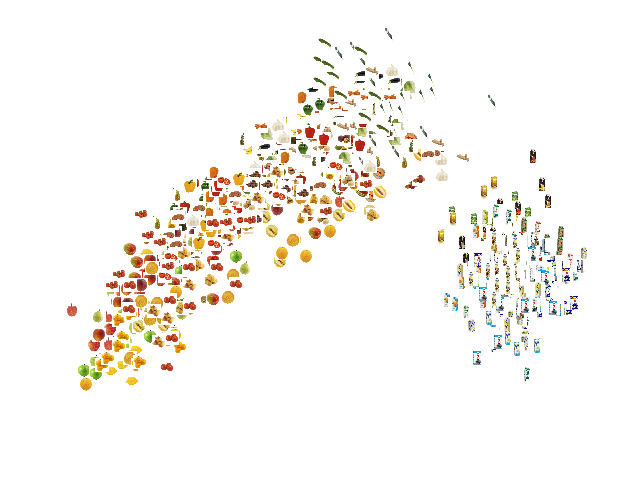
\includegraphics[width=\textwidth]{Chapter1/pics_paperB/pca_latents_vae_seed2}
	\vspace{-8mm}
	\caption{VAE$_{\vx}$}
	\label{fig:pca_latents_vae}
\end{subfigure}
\hfill
\begin{subfigure}[b]{0.3\textwidth}
	\centering
	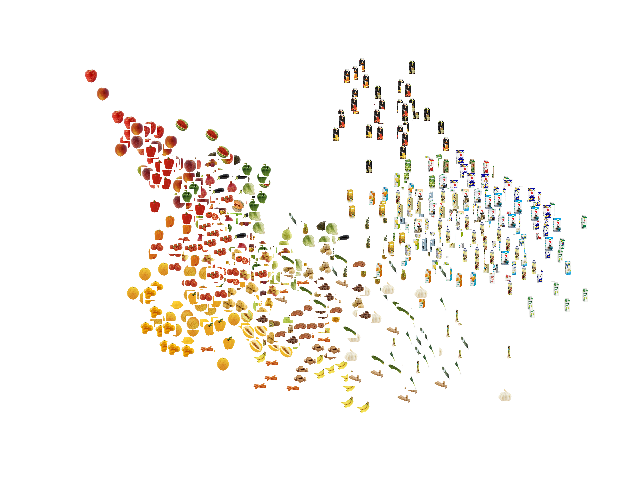
\includegraphics[width=\textwidth]{Chapter1/pics_paperB/pca_latents_vcca_xi_seed2}
	\vspace{-8mm}
	\caption{VCCA$_{\vx\vi}$}
\label{fig:pca_latents_vcca_xi}
\end{subfigure}
\hfill
\begin{subfigure}[b]{0.3\textwidth}
	\centering
	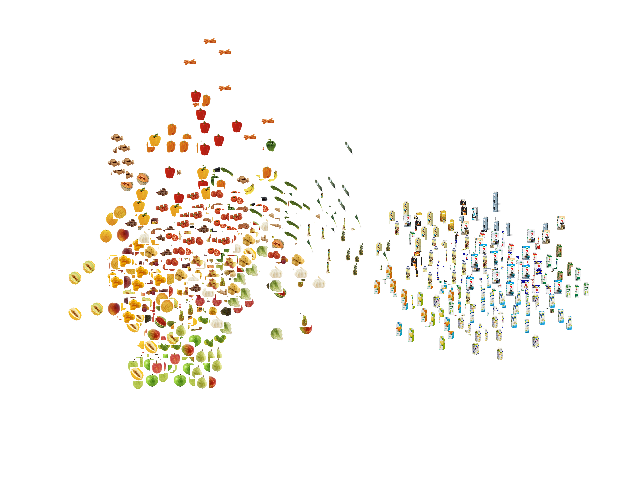
\includegraphics[width=\textwidth]{Chapter1/pics_paperB/pca_latents_vcca_xw_seed2}
	\vspace{-8mm}
	\caption{VCCA$_{\vx\vw}$}
\label{fig:pca_latents_vcca_xw}
\end{subfigure} \\ 
\begin{subfigure}[b]{0.3\textwidth}
	\centering
	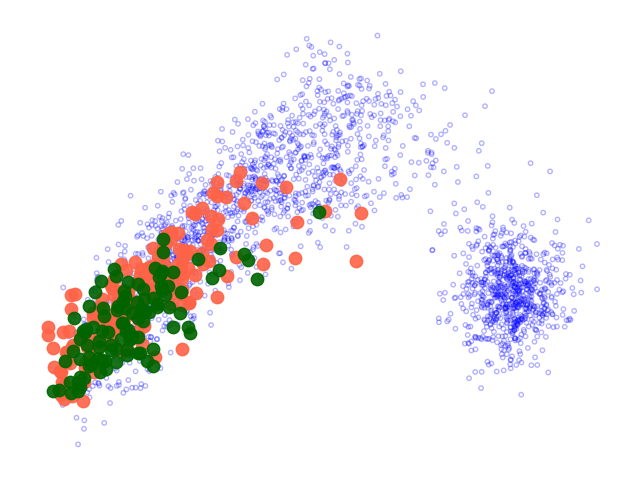
\includegraphics[width=\textwidth]{Chapter1/pics_paperB/pca_latents_apples_vae_seed2}
	\vspace{-8mm}
	\caption{VAE$_{\vx}$}
\label{fig:pca_latents_vae_apples}
\end{subfigure}
\hfill
\begin{subfigure}[b]{0.3\textwidth}
	\centering
	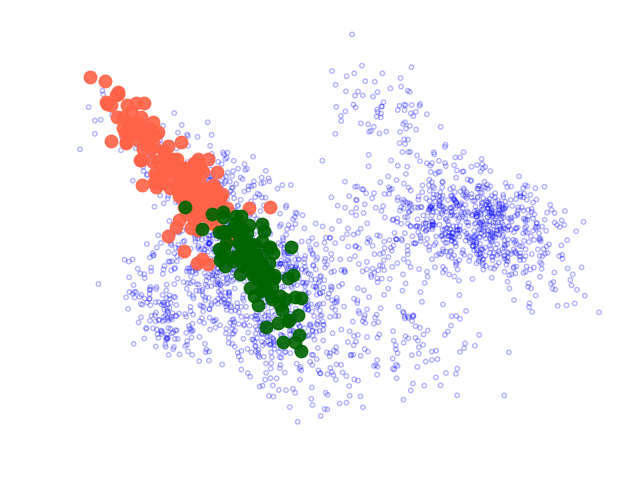
\includegraphics[width=\textwidth]{Chapter1/pics_paperB/pca_latents_apples_vcca_xi_seed2}
	\vspace{-8mm}
	\caption{VCCA$_{\vx\vi}$}
	\label{fig:pca_latents_vcca_xi_apples}
\end{subfigure}
\hfill
\begin{subfigure}[b]{0.3\textwidth}
	\centering
	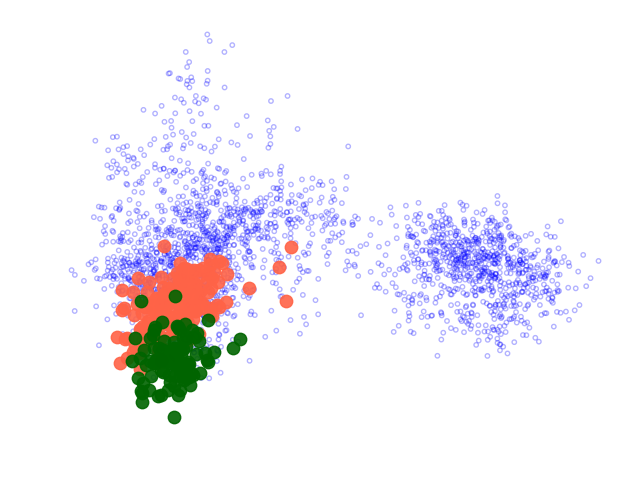
\includegraphics[width=\textwidth]{Chapter1/pics_paperB/pca_latents_apples_vcca_xw_seed2}
	\vspace{-8mm}
	\caption{VCCA$_{\vx\vw}$}
\label{fig:pca_latents_vcca_xw_apples}
\end{subfigure} \\
\begin{subfigure}[b]{0.3\textwidth}
	\centering
	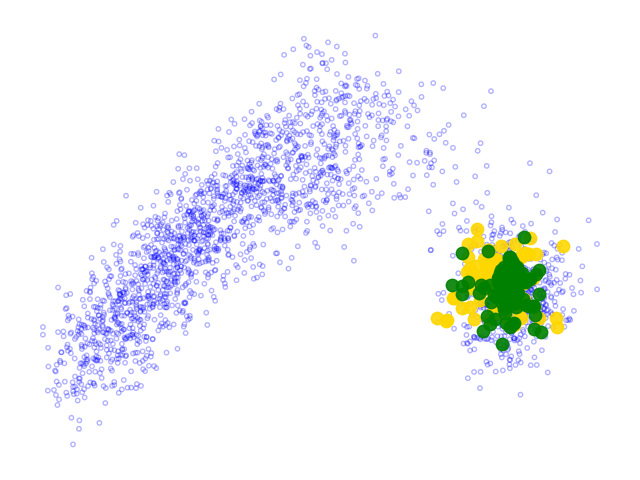
\includegraphics[width=\textwidth]{Chapter1/pics_paperB/pca_latents_juice_yoghurt_vae_seed2}
	\vspace{-8mm}
	\caption{VAE$_{\vx}$}
\label{fig:pca_latents_vae_juice_yoghurt}
\end{subfigure}
\hfill
\begin{subfigure}[b]{0.3\textwidth}
	\centering
	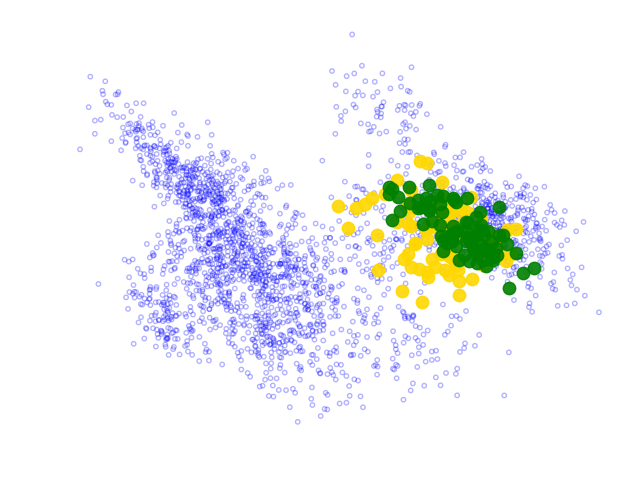
\includegraphics[width=\textwidth]{Chapter1/pics_paperB/pca_latents_juice_yoghurt_vcca_xi_seed2}
	\vspace{-8mm}
	\caption{VCCA$_{\vx\vi}$}
\label{fig:pca_latents_vcca_xi_juice_yoghurt}
\end{subfigure} 
\hfill
\begin{subfigure}[b]{0.3\textwidth}
	\centering
	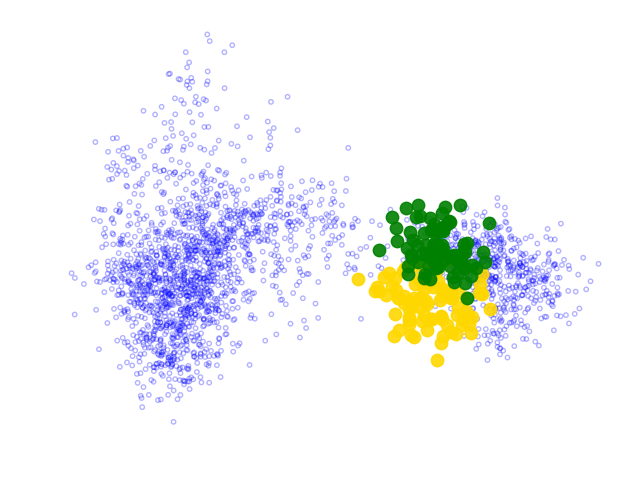
\includegraphics[width=\textwidth]{Chapter1/pics_paperB/pca_latents_juice_yoghurt_vcca_xw_seed2}
	\vspace{-8mm}
	\caption{VCCA$_{\vx\vw}$}
	\label{fig:pca_latents_vcca_xw_juice_yoghurt}
\end{subfigure}
	\vspace{-2mm}
	\caption{ Visualizations of the latent representations from VAE$_\vx$, VCCA$_{\vx\vi}$, and VCCA$_{\vx\vw}$ projected in 2-dimensional space with PCA. In (a-c), we show the latent representations plotted using the iconic images of the corresponding object class. In (d-f), we illustrate how the iconic images structures the items based on visual similarities by focusing on the \textcolor{ForestGreen}{green} and \textcolor{RedOrange}{red} apple classes in the dataset plotted in their corresponding colors. Similarly, in (g-i), we show how the text descriptions structure items based on ingredients and flavor by focusing on visually similar yoghurt (\textcolor{ForestGreen}{green}) and juice (\textcolor{GreenYellow}{yellow}) packages. The \textcolor{blue}{blue} dots correspond to all other grocery item classes. } 
	\label{fig:latent_space_visualizations}
	\vspace{-3mm}
\end{figure}

%Conclusions on visualizations: ​

%Iconic image structures items based on visual similarities​

%Text description structures items based on ingredients and flavor

\begin{wrapfigure}{r}{0.44\textwidth}
	\centering
	\vspace{-5mm}
	\begin{tabular}{c c c c}
		\hline \\[-5mm]
		\thead{\scriptsize Natural \\[-2mm] \scriptsize Image} & \thead{\scriptsize Iconic \\[-2mm] \scriptsize Image} & \thead{\scriptsize Decoded \\[-2mm] \scriptsize Image} \\[-1mm]
		%\scriptsize{{\bf Natural Image}} & \scriptsize{{\bf Iconic Image}} & \scriptsize{{\bf Decoded Image}}  \\
		\hline \\[-3mm]
		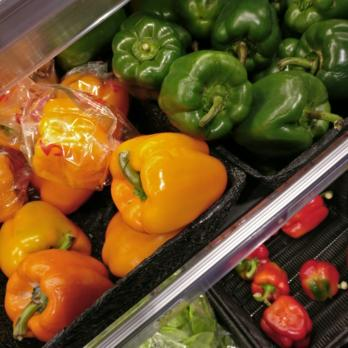
\includegraphics[width=13mm, height=13mm]{Chapter3/figures/decoded_iconic_images/Orange-Bell-Pepper_008.jpg} & 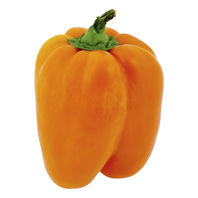
\includegraphics[width=13mm, height=13mm]{Chapter3/figures/iconic_image_figures/Orange-Bell-Pepper_Iconic.jpg} & 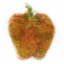
\includegraphics[width=13mm, height=13mm]{Chapter3/figures/decoded_iconic_images/vcca_xiwy/orange_bell_pepper_image2191.png}  \\[-0.7mm] 
		\hline \\[-3mm]
		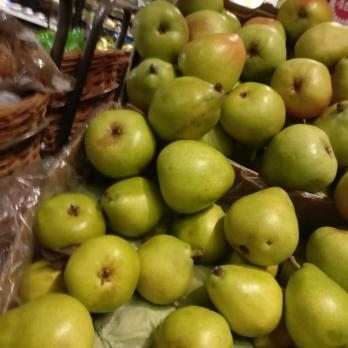
\includegraphics[width=13mm, height=13mm]{Chapter3/figures/decoded_iconic_images/Anjou_015.jpg} & 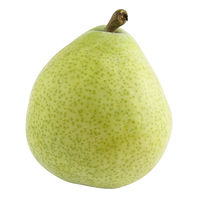
\includegraphics[width=13mm, height=13mm]{Chapter3/figures/iconic_image_figures/Anjou-Pear_Clean.jpg} & 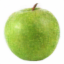
\includegraphics[width=13mm, height=13mm]{Chapter3/figures/decoded_iconic_images/vcca_xiwy/anjou_pear_image849.png} \\[-0.7mm]
		\hline
	\end{tabular}
	\vspace{-3mm}
	\captionsetup{width=.9\linewidth}
	\caption{Examples of decoded iconic images from VCCA$_{\vx \vi \vw \vy}$ with their corresponding natural image and true iconic image.}
	\vspace{-3mm}
	\label{fig:decoded_iconic_images}
\end{wrapfigure} 
\paragraph{Iconic Image Generation.} The iconic image decoder can provide explanations for the predicted classes. Figure \ref{fig:decoded_iconic_images} shows two examples of decoded iconic images from two natural images where the class labels are \textit{Orange Bell Pepper} and \textit{Anjou Pear}. On the first row, we see that VCCA$_{\vx \vi \vw \vy}$ has recognized the green bell peppers in the natural image and generated a mixed orange and green bell pepper in the iconic image. On the second row, we see that the decoded iconic image is a \textit{Granny Smith} apple instead of a pear which was the true class. The classifier consequently predicts the natural image to be a \textit{Granny Smith} apple. Hence, the iconic image decoder can be used as a tool for providing an intuition of why the classifier made an error. 



\section{Discussion}

In the experiments, we showed that utilizing the web-scraped information with VCCA can enhance the performance of grocery item classifiers. This shows that the cheaper web-scraped views can serve as a good alternative for improving classification performance over collecting more natural images in the grocery stores. Furthermore, we illustrated how the iconic images and text descriptions affects the structure of the latent space based on view-specific information. More specifically, the iconic images structures the latent space after visual similarities such as colors and shapes, while the text descriptions pushes items with similar ingredients and flavors closer to each other in the latent space. Finally, we demonstrated how the iconic images can be used for providing potential explanations for misclassifications, which could help us detect hard classes and give us indications of how robust the latent representations are to classifying images with different classes. 

We observed that utilizing the iconic images in VCCA affects the classification performance significantly better than the text descriptions. Potentially, this is due to the text description view to be more noisy than the iconic images as there are few words that are relevant to the recognition task. However, the text descriptions could be utilized more efficiently, for example by pre-processing the text to keep words describing fine-grained details about the items as well as removing stop words ('the', 'it', 'and', etc.) and other irrelevant words. A second option would be to use attention mechanisms~\cite{luong2015effective, vaswani2017attention} that helps the model to learn which words to emphasize on when learning the joint latent representations. We could also encode the text into a single-vector embedding with various methods~\cite{mikolov2013distributed, pennington2014glove, lan2019albert} and replace the RNN with an MLP predicting in the embedding space which the text embedding the natural image is closes to. 

Regarding the dataset collection, we have suggested extensions on how to provide more useful information about the items to improve the recognition task. Firstly, it would be valuable to download instances of iconic images and text descriptions from more supermarket websites to potentially allow the VCCA model to capture more view-specific variations into the learned representations. Secondly, the model should be extended to handle video data rather than still images. This would require record videos with the mobile phone camera in the grocery stores to properly evaluate the classifiers. Nevertheless, the extension to video would be beneficial for user experience of the recognition app since the classifier would receive more chances to classify the items correctly by utilizing multiple frames. 

Finally, the Grocery store dataset could be extended to zero/few-shot learning~\cite{xian2018zero, wang2020generalizing} and continual learning~\cite{delange2021continual, parisi2019continual} settings. Such applications are important for assistive vision devices to build data-efficient and adaptable systems that improves their usability in real-world scenarios. 



